\section{Tahapan Desain}
\label{sec:tahapan-desain}

\begin{figure}[htbp]
    \centering
    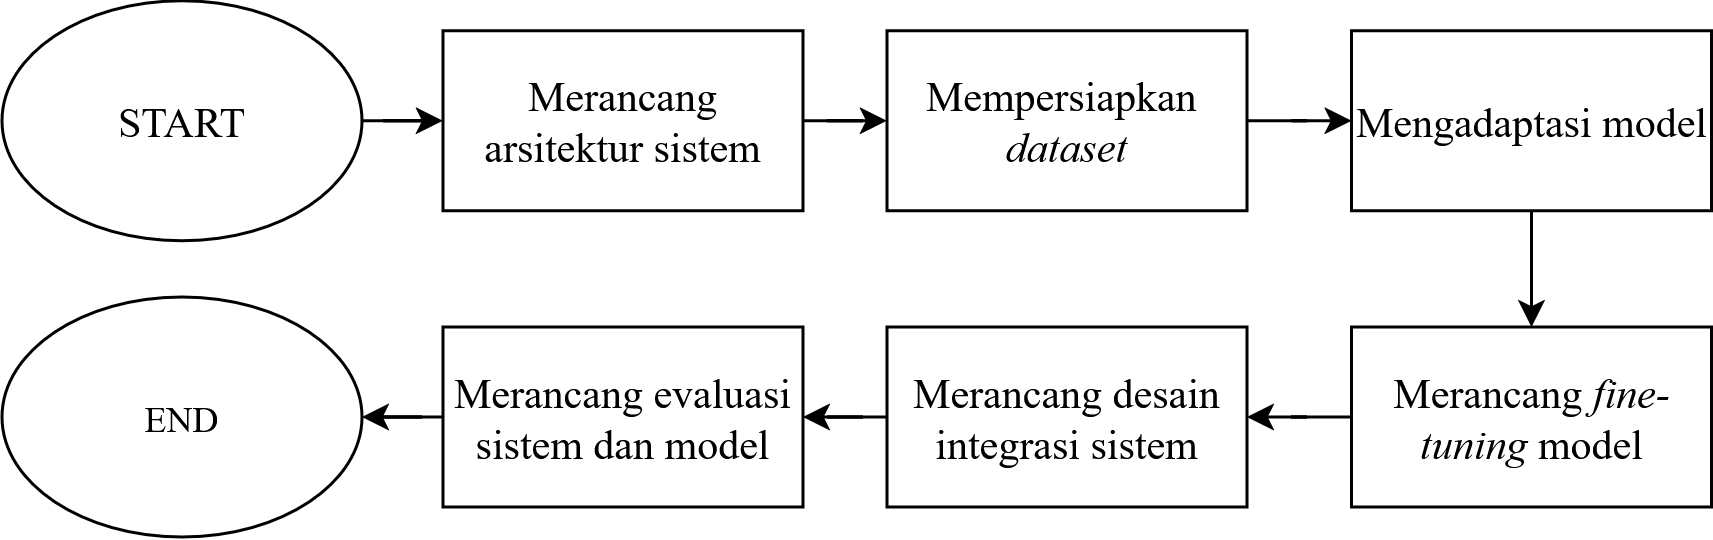
\includegraphics[width=\textwidth]{images/design-flow.png}
    \caption{Alur kerja tahapan desain sistem ekstraksi data struk dan bukti pembayaran}
    \label{fig:design-flow}
\end{figure}

\autoref{fig:design-flow} menunjukkan tahapan desain yang dilakukan dalam penelitian ini. Tahapan desain utama mencakup analisis kebutuhan dan arsitektur sistem, strategi persiapan dataset, pemilihan dan adaptasi model, perancangan \emph{fine-tuning}, desain integrasi sistem, dan perancangan metodologi evaluasi. Tahapan desain yang dihasilkan akan menjadi dasar untuk mengembangkan sistem ekstraksi data struk dan bukti pembayaran yang efektif dan efisien.

Proses desain dirancang dengan mempertimbangkan target pengguna Gen Z yang memiliki ekspektasi tinggi terhadap kemudahan penggunaan dan efisiensi sistem mobile. Setiap tahapan desain tidak hanya mempertimbangkan aspek teknis, tetapi juga pengalaman pengguna untuk memastikan sistem dapat diterima dan digunakan secara optimal oleh target pengguna. Tahapan desain dirancang berdasarkan alternatif solusi yang telah diusulkan pada \autoref{sec:analisis-pemilihan-solusi} dan disesuaikan dengan tahap desain pada metodologi \dsrm.

\subsection{Analisis Kebutuhan dan Arsitektur Sistem}
\label{subsec:analisis-kebutuhan-arsitektur}

Tahapan pertama dalam perancangan sistem adalah melakukan analisis kebutuhan dan merancang arsitektur sistem yang sesuai dengan tujuan penelitian. Berdasarkan analisis kebutuhan yang telah dilakukan pada \autoref{sec:analisis-kebutuhan}, sistem dirancang untuk memenuhi kebutuhan fungsional dan non-fungsional yang telah didefinisikan.

Arsitektur sistem dirancang menggunakan pendekatan \textit{client-server} dengan pemisahan yang jelas antara aplikasi \textit{mobile} sebagai \textit{frontend} dan layanan \textit{backend} untuk pemrosesan model. Keputusan untuk menggunakan arsitektur terdistribusi ini didasarkan pada kompleksitas model \donut{} yang memerlukan sumber daya komputasi tinggi dan tidak dapat dijalankan secara efisien pada perangkat \textit{mobile}.

% \begin{figure}[htbp]
%     \centering
%     \includegraphics[width=0.9\textwidth]{images/system-architecture.png}
%     \caption{Arsitektur sistem ekstraksi data pembayaran}
%     \label{fig:system-architecture}
% \end{figure}

\autoref{fig:system-architecture} menunjukkan arsitektur sistem yang terdiri dari tiga komponen utama: aplikasi \textit{mobile}, layanan API, dan modul pemrosesan model. Aplikasi \textit{mobile} berfungsi sebagai antarmuka pengguna untuk mengambil gambar, menampilkan hasil ekstraksi, dan mengelola data transaksi. Layanan API berperan sebagai penghubung antara aplikasi \textit{mobile} dan modul pemrosesan model, menangani \textit{request} dari klien dan mengembalikan hasil dalam format yang terstruktur.

Modul pemrosesan model mengimplementasikan dua model \donut{} yang berbeda: model \textit{QRIS-TF} untuk ekstraksi dan klasifikasi bukti pembayaran digital, dan model \textit{CORD-v2} untuk ekstraksi data dari struk pembayaran berbasis kertas. Pemilihan model dilakukan secara otomatis berdasarkan jenis dokumen yang diproses, memastikan setiap dokumen ditangani oleh model yang paling sesuai.

Arsitektur ini memberikan fleksibilitas dalam pengembangan dan pemeliharaan sistem, memungkinkan peningkatan model atau penambahan fitur baru tanpa mempengaruhi komponen lain. Selain itu, pendekatan terdistribusi memungkinkan sistem untuk menangani beban pemrosesan yang besar dan dapat diskalakan sesuai kebutuhan.


\subsection{Strategi Persiapan Dataset}
\label{subsec:strategi-persiapan-dataset}

Persiapan \dataset{} merupakan tahapan kritis dalam pengembangan sistem ekstraksi data pembayaran. Strategi persiapan \dataset{} dirancang untuk memastikan kualitas dan representativitas data yang akan digunakan untuk melatih model \donut{} yang telah disesuaikan dengan domain pembayaran Indonesia.

% \begin{figure}[htbp]
%     \centering
%     \includegraphics[width=0.8\textwidth]{images/data-preparation-flow.png}
%     \caption{Alur kerja persiapan dataset}
%     \label{fig:data-preparation-flow}
% \end{figure}

\autoref{fig:data-preparation-flow} menunjukkan alur kerja sistematis dalam persiapan \dataset. Proses dimulai dengan pengumpulan gambar bukti pembayaran dari berbagai sumber, termasuk aplikasi pembayaran digital (SeaBank, Neobank, BCA, \gopay) dan struk pembayaran berbasis kertas. Total \dataset{} yang dikumpulkan mencapai sekitar 300 gambar dengan distribusi yang seimbang antar jenis pembayaran.

Tahap anotasi data menggunakan pendekatan semi-otomatis dengan memanfaatkan \emph{Large Language Model} untuk menghasilkan anotasi awal yang kemudian diverifikasi dan diperbaiki secara manual. Format anotasi mengikuti standar JSONL dengan struktur yang konsisten untuk setiap jenis dokumen. Setiap sampel data mencakup informasi mengenai \emph{file path}, \emph{ground truth}, dan \emph{task identifier} yang sesuai dengan jenis dokumen.

Strategi pembagian \dataset{} menggunakan rasio 70:20:10 untuk data latih, validasi, dan uji. Pembagian ini dilakukan dengan mempertimbangkan distribusi jenis dokumen dan sumber data untuk memastikan representativitas setiap subset. Data latih digunakan untuk \emph{fine-tuning} model, data validasi untuk monitoring proses pelatihan dan \emph{early stopping}, sedangkan data uji digunakan untuk evaluasi akhir kinerja model.

Validasi kualitas \dataset{} dilakukan melalui proses \emph{quality check} yang mencakup verifikasi format anotasi, konsistensi label, dan kualitas gambar. Sampel data yang tidak memenuhi standar kualitas akan diperbaiki atau dihapus dari \dataset{} untuk memastikan integritas data pelatihan. Pendekatan sistematis ini memastikan bahwa model akan dilatih dengan data berkualitas tinggi yang representatif terhadap variasi dokumen pembayaran yang ada di Indonesia.


\subsection{Pemilihan dan Adaptasi Model}
\label{subsec:pemilihan-adaptasi-model}

Pemilihan model merupakan keputusan strategis yang menentukan keberhasilan sistem ekstraksi data pembayaran. Berdasarkan analisis pemilihan solusi pada \autoref{sec:analisis-pemilihan-solusi}, \donut{} dipilih sebagai model utama karena pendekatan \emph{end-to-end} yang tidak memerlukan \ocr{} dan kemampuannya dalam memahami dokumen semi-terstruktur.

% \begin{figure}[htbp]
%     \centering
%     \includegraphics[width=0.7\textwidth]{images/model-selection-tree.png}
%     \caption{Pohon keputusan pemilihan model berdasarkan jenis dokumen}
%     \label{fig:model-selection-tree}
% \end{figure}

Strategi adaptasi model menggunakan pendekatan \emph{dual-model} yang disesuaikan dengan karakteristik dokumen yang berbeda. \autoref{fig:model-selection-tree} menunjukkan logika pemilihan model berdasarkan jenis dokumen input. Untuk dokumen pembayaran digital (QRIS dan transfer), sistem menggunakan model yang di-\emph{fine-tune} khusus pada \dataset{} QRIS-TF yang mampu melakukan ekstraksi sekaligus klasifikasi jenis pembayaran. Sedangkan untuk struk pembayaran berbasis kertas, sistem menggunakan model yang di-\emph{fine-tune} pada \dataset{} CORD-v2 yang fokus pada ekstraksi informasi tanpa klasifikasi.

Model \textit{QRIS-TF} dirancang untuk menangani kompleksitas dokumen pembayaran digital yang memiliki variasi layout dan format dari berbagai aplikasi pembayaran. Model ini tidak hanya mengekstraksi informasi seperti nominal pembayaran, waktu transaksi, dan identifikator transaksi, tetapi juga mengklasifikasikan jenis transaksi (QRIS atau transfer). Kemampuan klasifikasi terintegrasi ini menghilangkan kebutuhan untuk langkah pemrosesan tambahan dan meningkatkan efisiensi sistem secara keseluruhan.

Model \textit{CORD-v2} dioptimalkan untuk menangani struk pembayaran berbasis kertas yang memiliki karakteristik visual yang berbeda dari dokumen digital. Fokus pada ekstraksi informasi memungkinkan model ini mencapai akurasi tinggi dalam mengenali elemen-elemen penting seperti nama toko, total pembayaran, dan detail item pembelian.

Adaptasi kedua model dilakukan melalui ekspansi kosakata dengan menambahkan \emph{special tokens} yang spesifik untuk domain pembayaran Indonesia. \emph{Special tokens} ini mencakup representasi untuk mata uang rupiah, format tanggal Indonesia, dan terminologi pembayaran lokal. Proses adaptasi juga melibatkan penyesuaian \emph{task prompt} yang mengarahkan model untuk menghasilkan output dalam format yang konsisten dengan kebutuhan sistem.


\subsection{Perancangan Fine-tuning}
\label{subsec:perancangan-fine-tuning}

Perancangan strategi \emph{fine-tuning} merupakan tahapan kritis yang menentukan kualitas adaptasi model terhadap domain pembayaran Indonesia. Strategi ini dirancang untuk mengoptimalkan kinerja model sambil mencegah \emph{overfitting} dan memastikan efisiensi komputasi.

% \begin{figure}[htbp]
%     \centering
%     \includegraphics[width=0.8\textwidth]{images/training-process-flow.png}
%     \caption{Alur kerja proses fine-tuning model}
%     \label{fig:training-process-flow}
% \end{figure}

\autoref{fig:training-process-flow} menggambarkan proses \emph{fine-tuning} yang sistematis, dimulai dari inisialisasi model dasar hingga penyimpanan model yang telah dilatih. Proses ini dirancang dengan mempertimbangkan karakteristik \dataset{} dan sumber daya komputasi yang tersedia.

Konfigurasi pelatihan ditetapkan berdasarkan praktik terbaik dalam \emph{fine-tuning} model \transformer{} untuk tugas pemahaman dokumen. Jumlah \emph{epoch} ditetapkan sebanyak 30 berdasarkan beberapa pertimbangan utama. Pertama, penelitian pada model \donut{} menunjukkan bahwa konvergensi optimal untuk tugas \emph{fine-tuning} umumnya tercapai dalam rentang 20-40 \emph{epoch} \parencite{kim2021donut}. Kedua, dengan ukuran \dataset{} sekitar 300 sampel, 30 \emph{epoch} memberikan sekitar 10.000 iterasi parameter update yang sufficient untuk adaptasi domain tanpa risiko \emph{overfitting} yang signifikan. Ketiga, implementasi \emph{early stopping} dengan \emph{patience}=3 memungkinkan penghentian pelatihan secara otomatis jika tidak ada peningkatan pada \emph{validation loss} selama 3 \emph{epoch} berturut-turut, mencegah pemborosan sumber daya komputasi.

Strategi optimasi menggunakan \emph{batch size} 1 dengan \emph{gradient accumulation} sebanyak 8 langkah untuk mensimulasikan efek \emph{batch size} yang lebih besar sambil mengakomodasi keterbatasan memori GPU. \emph{Learning rate} ditetapkan pada 3e-5 sebagai titik optimal antara kecepatan konvergensi dan stabilitas pelatihan. Penggunaan \emph{mixed precision} FP16 memungkinkan pelatihan yang lebih efisien secara memori tanpa mengorbankan akurasi model.

Monitoring pelatihan dilakukan melalui pelacakan metrik validasi secara berkala, termasuk \emph{loss}, akurasi, dan metrik evaluasi khusus seperti \mcer. Implementasi \emph{checkpoint} otomatis setiap 5 \emph{epoch} memastikan bahwa progres pelatihan tidak hilang jika terjadi gangguan sistem. Strategi ini juga memungkinkan analisis evolusi kinerja model sepanjang proses pelatihan dan pemilihan \emph{checkpoint} optimal berdasarkan kinerja validasi.

Validasi robustness model dilakukan melalui evaluasi pada \dataset{} validasi yang mencakup berbagai variasi dokumen pembayaran. Proses ini memastikan bahwa model tidak hanya menghasilkan akurasi tinggi pada data pelatihan, tetapi juga mampu generalisasi dengan baik pada data yang belum pernah dilihat sebelumnya.


\subsection{Desain Integrasi Sistem}
\label{subsec:desain-integrasi-sistem}

Desain integrasi sistem bertujuan untuk menciptakan komunikasi yang seamless antara komponen-komponen sistem, mulai dari aplikasi \textit{mobile} hingga model pemrosesan di \textit{backend}. Integrasi dirancang dengan mempertimbangkan efisiensi, reliabilitas, dan kemudahan penggunaan bagi pengguna Gen Z.

% \begin{figure}[htbp]
%     \centering
%     \includegraphics[width=0.9\textwidth]{images/system-integration-flow.png}
%     \caption{Alur integrasi sistem end-to-end}
%     \label{fig:system-integration-flow}
% \end{figure}

\autoref{fig:system-integration-flow} menunjukkan alur integrasi yang menghubungkan seluruh komponen sistem. Komunikasi antara aplikasi \textit{mobile} dan \textit{backend service} menggunakan protokol HTTP/HTTPS dengan format data \json{} untuk memastikan kompatibilitas dan kemudahan parsing. Desain API mengikuti prinsip \textit{RESTful} dengan \textit{endpoint} yang jelas dan konsisten untuk setiap operasi.

Aplikasi \textit{mobile} dirancang dengan dua mekanisme utama untuk input gambar: pengambilan foto langsung menggunakan kamera dan integrasi dengan sistem \textit{sharing} Android. Sistem \textit{sharing} memungkinkan pengguna untuk membagikan \emph{screenshot} bukti pembayaran dari aplikasi lain secara langsung ke aplikasi TrackMyBills, menciptakan pengalaman pengguna yang natural dan efisien. Mekanisme ini particularly important untuk target pengguna Gen Z yang terbiasa dengan interaksi mobile yang intuitif.

Proses pemilihan model dilakukan secara otomatis di sisi \textit{backend} berdasarkan analisis karakteristik gambar input. Sistem menggunakan heuristik sederhana yang mengidentifikasi pola visual untuk menentukan apakah dokumen merupakan bukti pembayaran digital atau struk berbasis kertas. Pendekatan ini menghilangkan kebutuhan pengguna untuk secara manual memilih jenis dokumen, menyederhanakan \textit{user flow} dan mengurangi potensi kesalahan.

Desain \textit{error handling} dan \textit{fallback mechanism} memastikan sistem tetap responsif bahkan ketika terjadi kegagalan pada salah satu komponen. Jika model utama gagal memproses dokumen, sistem secara otomatis mencoba menggunakan model alternatif atau memberikan respon yang informatif kepada pengguna. Implementasi \textit{timeout} yang sesuai mencegah aplikasi \textit{mobile} menunggu terlalu lama untuk respons dari \textit{backend}.

Keamanan komunikasi dijamin melalui validasi input yang ketat, sanitasi data, dan implementasi \textit{rate limiting} untuk mencegah penyalahgunaan sistem. Format respons dirancang konsisten dengan menyertakan metadata yang membantu aplikasi \textit{mobile} dalam menampilkan hasil ekstraksi dengan cara yang user-friendly. Desain ini memastikan bahwa integrasi sistem tidak hanya berfungsi secara teknis, tetapi juga memberikan pengalaman pengguna yang optimal.


\subsection{Perancangan Metodologi Evaluasi}
\label{subsec:perancangan-metodologi-evaluasi}

Perancangan metodologi evaluasi dirancang untuk memberikan penilaian komprehensif terhadap sistem ekstraksi data pembayaran, mencakup aspek teknis dan pengalaman pengguna. Metodologi ini dirancang dengan pendekatan multi-dimensional yang memisahkan evaluasi kinerja model dan evaluasi usabilitas sistem.

% \begin{figure}[htbp]
%     \centering
%     \includegraphics[width=0.8\textwidth]{images/evaluation-framework.png}
%     \caption{Framework evaluasi sistem secara komprehensif}
%     \label{fig:evaluation-framework}
% \end{figure}

\autoref{fig:evaluation-framework} menggambarkan struktur evaluasi yang terbagi menjadi dua cabang utama: evaluasi kinerja model dan evaluasi usabilitas sistem. Pendekatan terpisah ini memungkinkan analisis yang mendalam terhadap aspek teknis dan human-computer interaction secara independen, sambil tetap memberikan gambaran holistik tentang kualitas sistem.

Evaluasi kinerja model dirancang untuk mengukur akurasi ekstraksi data dan klasifikasi dokumen menggunakan metrik standar industri. Metrik yang digunakan mencakup \accuracy{}, \precision{}, \recall{}, F1-\emph{score}, dan \mcer{} dengan ambang batas minimum yang telah ditetapkan berdasarkan standar penelitian terdahulu. \accuracy{}, \precision{}, \recall{}, dan F1-\emph{score} ditetapkan dengan ambang minimum 70\% berdasarkan standar untuk sistem pemahaman dokumen \parencite{kim2021donut, xu2020layoutlm}. \mcer{} ditetapkan dengan ambang maksimum 20\% sebagai indikator akurasi ekstraksi teks yang dapat diterima \parencite{holley2009ocr}.

Implementasi evaluasi model menggunakan pendekatan \emph{unified evaluation} yang dapat menangani kedua jenis model (QRIS-TF dan CORD-v2) dalam satu framework. Sistem evaluasi dirancang dengan fleksibilitas untuk menghitung metrik yang sesuai dengan karakteristik masing-masing model, termasuk evaluasi klasifikasi untuk model QRIS-TF dan fokus ekstraksi untuk model CORD-v2.

Evaluasi usabilitas menggunakan instrumen SUS \emph{score} untuk mengukur pengalaman pengguna Gen Z dalam menggunakan aplikasi mobile. Sampel evaluasi ditetapkan minimum 8 pengguna Gen Z untuk memastikan reliabilitas hasil. Ambang batas SUS ditetapkan pada skor 68 sebagai indikator usabilitas yang dapat diterima, dengan target skor 80+ untuk usabilitas yang excellent \parencite{bangor2009determining}.

Desain protokol evaluasi mencakup skenario penggunaan yang realistis, di mana pengguna diminta untuk memproses berbagai jenis dokumen pembayaran dan memberikan penilaian terhadap kemudahan penggunaan sistem. Evaluasi dilakukan dalam kondisi yang mensimulasikan penggunaan sehari-hari, termasuk variasi kualitas gambar dan jenis dokumen yang beragam.

Metodologi evaluasi juga dirancang untuk mengidentifikasi korelasi antara kinerja teknis dan persepsi pengguna. Analisis ini penting untuk memvalidasi bahwa peningkatan akurasi model berkontribusi terhadap peningkatan kepuasan pengguna. Pendekatan evaluasi yang comprehensive ini memastikan bahwa sistem tidak hanya unggul secara teknis, tetapi juga memberikan nilai praktis bagi pengguna dalam kehidupan sehari-hari.
